%SECTION%%%%%%%%%%%%%%%%%%%
\section[Tricks]{3. Tricks of the Trade}
\begin{frame}
\small{\frametitle{Outline}
\tableofcontents
}
\end{frame}
%%%%%%%%%%%%%%%%%%%%


%% SUBSECTION%%%%%
\subsection[Optimization]{Optimization: Making SGD work, Adaptive Learning Rate, 2nd-order methods}

%%%%%%
\begin{frame}
\frametitle{Neural Net Training Recipe}
\centerline{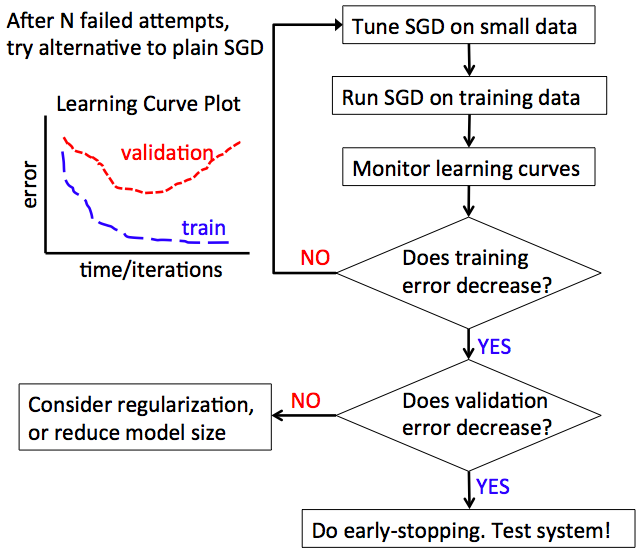
\includegraphics[scale=0.42]{figs/training_recipe}}
\end{frame}

%%%%%%
\begin{frame}
\frametitle{Making plain SGD Work}
\bi
\item With some tuning, SGD often works just as well as more advanced optimization methods! \pause
\item Important hyper-parameters: 
	\bi
	\item Learning rate: tune on small data first
	\item Mini-batch size: fit to computer's memory
	\ei 
	\pause
\item General tips:
	\bi
	\item Shuffle training data
	\item Scale training data within suitable range 
	\item Randomly initialize weights, e.g. uniform$[-1/\sqrt{(FanIn)}, 1/\sqrt{(FanIn)}]$
	\ei
\ei	
\end{frame}


%%%%%%%%%%%%%
\begin{frame}
\frametitle{Effect of Learning Rate $\gamma$ on SGD Convergence}
\bi
\item Update: $w \leftarrow w - \gamma( \sum_m {\color{red} Error^{(m)}} * {\color{blue} \sigma'(in^{(m)})} * x^{(m)
})$
\bi
        \item $\gamma$: try to be as large as possible without divergence.
        \item Common heuristic: $\gamma_t = \frac{\gamma_0}{1 + \gamma_0 * \lambda * t} = O(1/t)$ 
\ei
\item Analysis by \cite{schaul13learningrate} (in plot, $\eta \equiv \gamma$):
\ei
\centerline{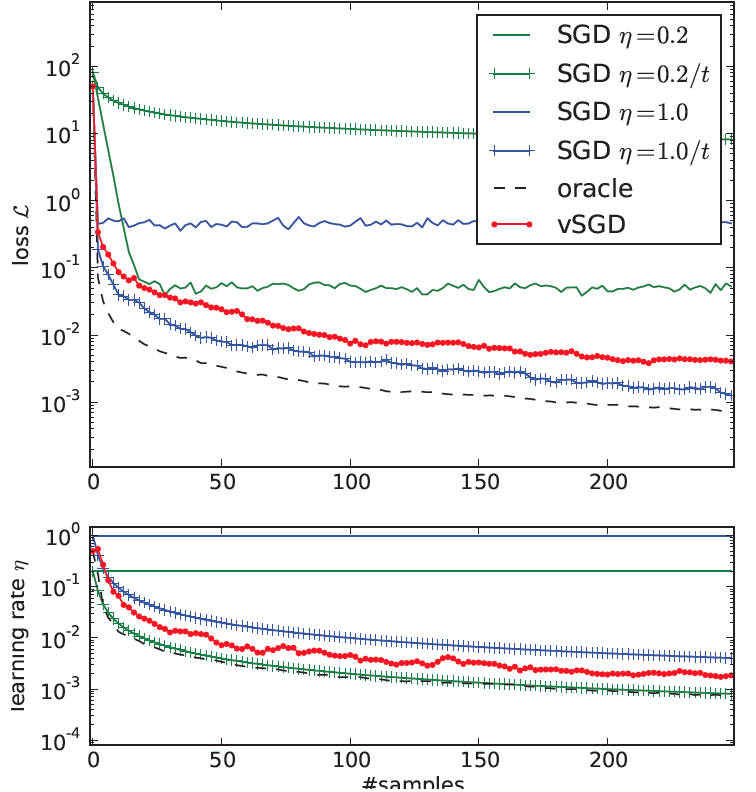
\includegraphics[scale=0.23]{figs/schaul13learningrate}}
\end{frame}


%%%%
\begin{frame}
\frametitle{Difficulty of optimizing highly non-convex loss functions}
\bi
\item "Pathological curvature" is tough to navigate for SGD 
\item Many methods for avoiding this zig-zag problem.
\ei
\centerline{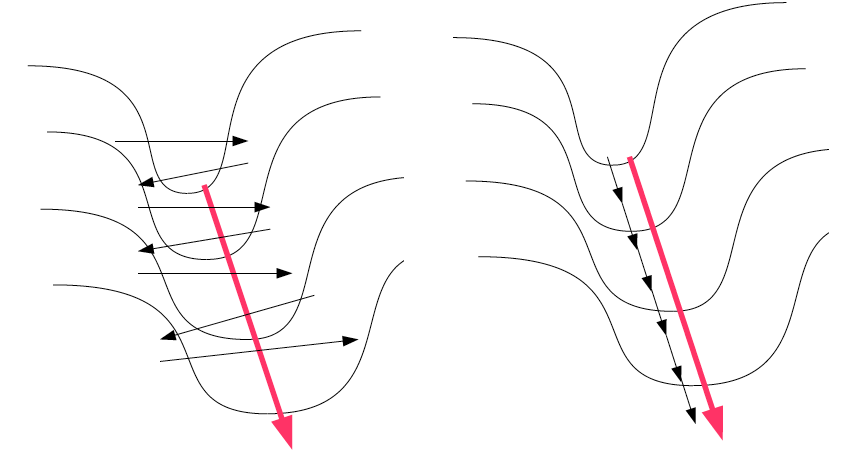
\includegraphics[scale=0.36]{figs/gradient_vs_newton}}
\blfootnote{Figure from \cite{martens10hessianfree}}
\end{frame}

%%%%%%
\begin{frame}
\frametitle{SGD + Momentum}
\bi
\item Idea: Accelerate in the direction that is consistently pointed to by successive gradients
\pause
\item Let update equation be: $w_{t+1} = w_t + \Delta w_t$
	\bi
	\item SGD: $\Delta w_t = -\gamma g_t$, where $g_t$ is gradient
	\pause
	\item SGD+Momemtum: $\Delta w_t = \rho \Delta w_{t-1} - \gamma g_t$ \pause
	\ei
\item $\rho$: a constant that determines how much momentum from previous updates \pause
\item Zig-zag directions will be cancelled out, while others will be accelerated.
\ei
\blfootnote{Note slight change of notation in this section: $w$ is a vector of weights, subscript $t$ in $w_t$ refers to weight at time $t$, not index as in previous sections}
\end{frame}

%%%%%%
\begin{frame}
\frametitle{Adaptive Learning Rate: ADAGRAD \cite{duchi11adagrad}}
\bi
\item Idea: 
	\bi 
	\item Each individual weight has it's own dynamic learning rate. 
	\item Weights with large derivative have smaller learning rate, weights with small derivative have large learning rate $\rightarrow$ different scales are balanced
	\ei
\item Let update equation be: $w_{t+1} = w_t + \Delta w_t$
	\bi
	\item SGD: $\Delta w_t = -\gamma g_t$, where $g_t$ is gradient
	\item ADAGRAD: $\Delta w_t = - \frac{\gamma}{diag(\sqrt{\sum_{\tau=1}^t g_\tau g_\tau^T})} g_t$
	\ei 
\item Denominator accumulates the $\ell_2$ norm of past gradients per dimension. 
\ei
\end{frame}

%%%%%%
\begin{frame}
\frametitle{Adaptive Learning Rate: ADADELTA \cite{zeiler12adadelta}}
\bi
\item Idea: Similar to ADAGRAD, but no learning rate.
	\bi
	\item ADAGRAD: $\Delta w_t = - \frac{\gamma}{diag(\sqrt{\sum_{\tau=1}^t g_\tau g_\tau^T})} g_t$
	\ei
\item ADADELTA: 
	\be
	\item Accumulate gradient over sliding window: $E[g^2]_t = \rho E[g^2]_{t-1} + (1-\rho) g_t g_t^T$\\[0.2cm]
	\item $\Delta w_t = - \frac{RMS(E[\Delta w]_{t-1})}{RMS(E[g^2]_t)} g_t$\\[0.2cm]
	 where $RMS(E[g^2]_t) = \sqrt{E[g^2]_t + \epsilon}$\\[0.2cm]
	\item Accumulate update over sliding window: $E[\Delta w^2]_t = \rho E[\Delta w^2]_{t-1} + (1-\rho) \Delta w_t \Delta w_t^T$
	\ee
\ei
\end{frame}

\begin{frame}
\frametitle{2nd-order (Newton) methods}
\bi
\item Idea: approximate the loss function locally with a quadratic\\[0.2cm]
$L(w+z) \approx q_w(z) \equiv L(w) + \nabla L(w)^T z + \frac{1}{2} z^T H z $\\[0.2cm]
\hspace{1cm} where $H$ is the Hessian (curvature matrix) at $w$\\[0.2cm]
\pause
\item Minimizing this gives the search direction: $z^{*}=-H^{-1}\nabla L(w) $
        \bi
        \item Intuitively, $H^{-1}$ fixes any pathological curvature for $\nabla L(w)$
        \item In practice, don't want to store nor invert $H$
        \ei
\pause
\item Quasi-Newton methods
        \bi
        \item L-BFGS: uses low-rank approximation of $H^{-1}$
        \pause
        \item Hessian-free (i.e. truncated Newton): (1) minimize $q_w(z)$ with conjugate gradient method; (2) computes $Hz$ directly using finite-difference: $Hz = \lim_{\epsilon\rightarrow 0} \frac{\nabla L(w+\epsilon z) - \nabla L(w)}{\epsilon}$
        \ei
\ei
\end{frame}

\begin{frame}
\frametitle{Hessian-free optimization results}
\bi
\item Experiments in \cite{martens10hessianfree} \\[0.2cm]
\begin{center}
(Random initialization + 2nd-order Hessian-free optimizer) \\[0.2cm]
 gives lower training error than \\[0.2cm]
 (Pre-training initialization + 1-order optimizer).\\[0.5cm]
 \end{center}
 \item Nice results in Recurrent Nets too \cite{martens11recurrent}
\ei
\end{frame}

%% SUBSECTION%%%%%
\subsection[Regularization]{Regularization: Dropout, Multi-task learning}


%%%%%%%%%%%%%%%%
\begin{frame}
\frametitle{Dropout \cite{hinton12dropout}}
\begin{columns}
\begin{column}{0.5\textwidth}
\bi
\item Each time we present $x^{(m)}$, randomly delete each hidden node with 0.5 probability
\item This is like sampling from $2^{|h|}$ different architectures
\item At test time, use all nodes but halve the weights
\item Effect: Reduce overfitting by preventing "co-adaptation"; ensemble model averaging
\ei
\end{column}
\begin{column}{0.5\textwidth}
\begin{center}
\begin{tikzpicture}[->,>=stealth',shorten >=1pt,auto,node distance=3cm,
  thick,main node/.style={circle,fill=blue!20,draw,font=\sffamily\Large\bfseries},cross/.style={path picture={
  \draw[red]
(path picture bounding box.south east) -- (path picture bounding box.north west) (path picture bounding box.south west) -- (path picture bounding box.north east);
}}]

 \node[main node] (x1) at (0,0) {$x_1$};
  \node[main node] (x2) at (2,0) {$x_2$};
  \node[main node] (x3) at (4,0) {$x_3$};
  \node[main node] (h1) at (0,2) {$h_1$};
  \node[main node] (h2) at (2,2) {$h_2$};
  \node[main node] (h3) at (4,2) {$h_3$};
  \node[main node] (h'1) at (0,4) {$h'_1$};
  \node[main node] (h'2) at (2,4) {$h'_2$};
  \node[main node] (h'3) at (4,4) {$h'_3$};
  \node[main node] (y) at (2,6) {$y$};
   \node [draw,circle,cross,minimum width=1 cm] at (0,2){};
   \node [draw,circle,cross,minimum width=1 cm] at (2,4){};
   \node [draw,circle,cross,minimum width=1 cm] at (4,4){};


  \path[every node/.style={font=\sffamily\small}]
    (x1) edge node {} (h1)
    (x1) edge node {} (h2)
    (x1) edge node {} (h3)
    (x2) edge node {} (h1)
    (x2) edge node {} (h2)
    (x2) edge node {} (h3)
    (x3) edge node {} (h1)
    (x3) edge node {} (h2)
    (x3) edge node {} (h3)
    (h1) edge node {} (h'1)
    (h1) edge node {} (h'2)
    (h1) edge node {} (h'3)
    (h2) edge node {} (h'1)
    (h2) edge node {} (h'2)
    (h2) edge node {} (h'3)
    (h3) edge node {} (h'1)
    (h3) edge node {} (h'2)
    (h3) edge node {} (h'3)
    
      (h'1) edge node {} (y)
    (h'2) edge node {} (y)
    (h'3) edge node {} (y) ;

\end{tikzpicture}
\end{center}
\end{column}
\end{columns}
\end{frame}

%%%%%%%%%%%%%%%%
\begin{frame}
\frametitle{Dropout \cite{hinton12dropout}}
\begin{columns}
\begin{column}{0.5\textwidth}
\bi
\item Each time we present $x^{(m)}$, randomly delete each hidden node with 0.5 probability
\item This is like sampling from $2^{|h|}$ different architectures
\item At test time, use all nodes but halve the weights
\item Effect: Reduce overfitting by preventing "co-adaptation"; ensemble model averaging
\ei
\end{column}
\begin{column}{0.5\textwidth}
\begin{center}
\begin{tikzpicture}[->,>=stealth',shorten >=1pt,auto,node distance=3cm,
  thick,main node/.style={circle,fill=blue!20,draw,font=\sffamily\Large\bfseries},cross/.style={path picture={
  \draw[red]
(path picture bounding box.south east) -- (path picture bounding box.north west) (path picture bounding box.south west) -- (path picture bounding box.north east);
}}]

 \node[main node] (x1) at (0,0) {$x_1$};
  \node[main node] (x2) at (2,0) {$x_2$};
  \node[main node] (x3) at (4,0) {$x_3$};
  \node[main node] (h1) at (0,2) {$h_1$};
  \node[main node] (h2) at (2,2) {$h_2$};
  \node[main node] (h3) at (4,2) {$h_3$};
  \node[main node] (h'1) at (0,4) {$h'_1$};
  \node[main node] (h'2) at (2,4) {$h'_2$};
  \node[main node] (h'3) at (4,4) {$h'_3$};
  \node[main node] (y) at (2,6) {$y$};
   \node [draw,circle,cross,minimum width=1 cm] at (0,2){};
   \node [draw,circle,cross,minimum width=1 cm] at (2,4){};
   \node [draw,circle,cross,minimum width=1 cm] at (4,4){};


  \path[every node/.style={font=\sffamily\small}]
    (x1) edge node {} (h2)
    (x1) edge node {} (h3)
    (x2) edge node {} (h2)
    (x2) edge node {} (h3)
    (x3) edge node {} (h2)
    (x3) edge node {} (h3)
    (h2) edge node {} (h'1)
    (h3) edge node {} (h'1)
      (h'1) edge node {} (y)
  ;

\end{tikzpicture}
\end{center}
\end{column}
\end{columns}
\end{frame}


\begin{frame}
\frametitle{Some Results: TIMIT phone recognition}
\centerline{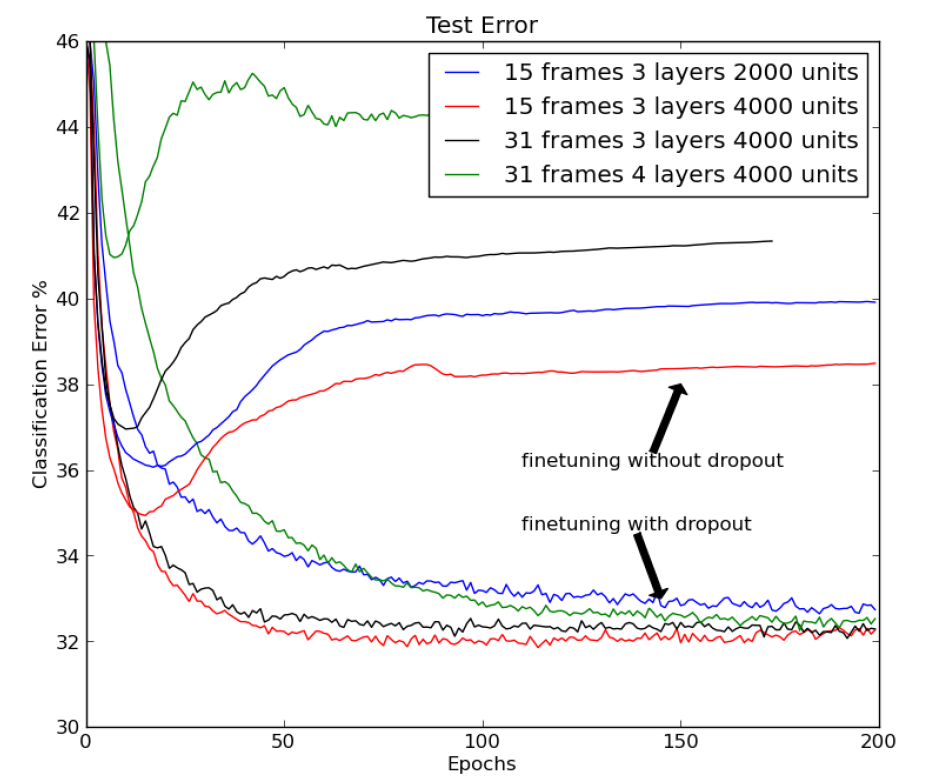
\includegraphics[scale=0.3]{figs/dropout_timit}}
\end{frame}

%%%%
\begin{frame}
\frametitle{Multi-task Learning: sharing hidden layers }
\bi
\item If too data is insufficient for desired task: 
\be
	\item train jointly with related tasks with shared hidden layer
	\item use related tasks' hidden layer as feature representation
\ee
\item e.g. \cite{liu15multitask}
\ei
\centerline{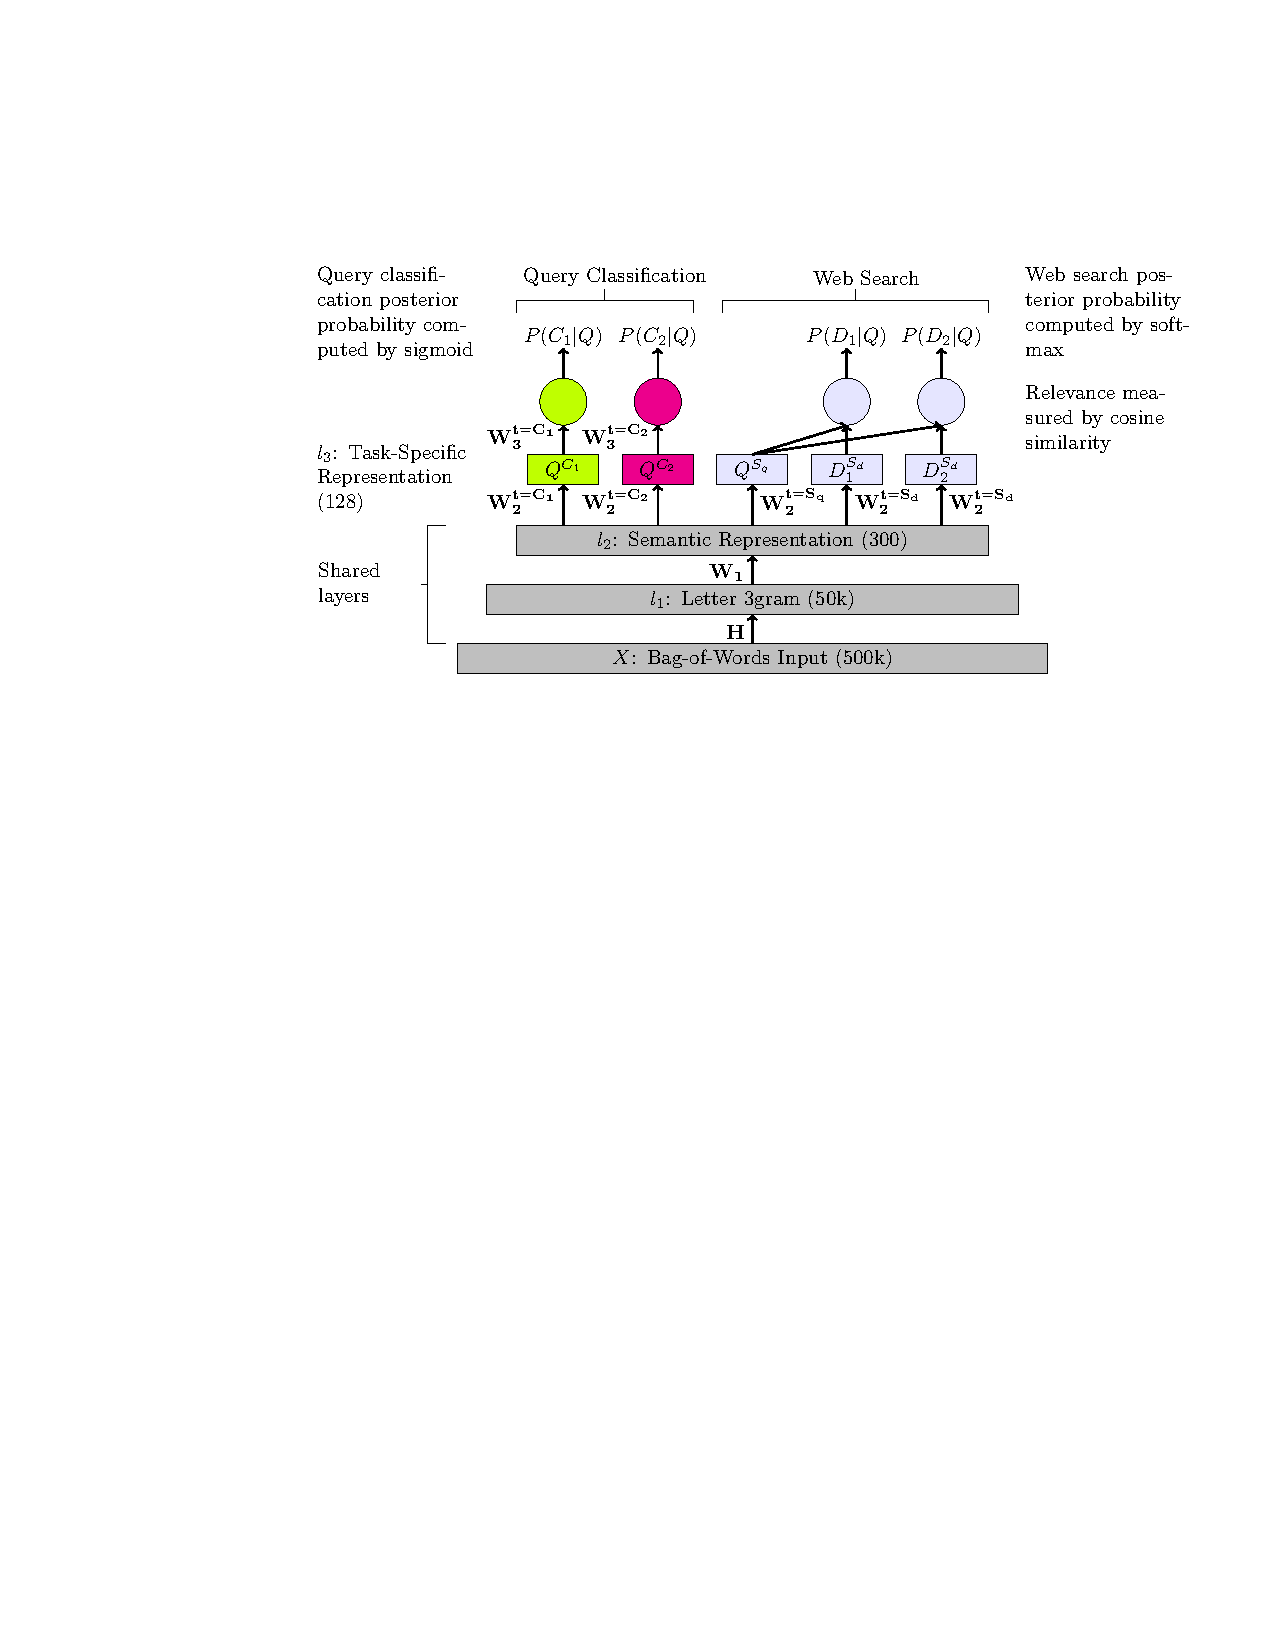
\includegraphics[scale=0.7]{figs/liu15multitask_mtdnn_arch}}
\blfootnote{See also \cite{caruana97,collobert11scratch,bordes12joint}}
\end{frame}

%%%%
\begin{frame}[plain]
\frametitle{Multi-task learning results in \cite{liu15multitask}}

\begin{table}
\centering
\tabcolsep=0.08cm
\begin{tabular}{|c | c | c | c | c || c | }
\hline
\multirow{2}{*}{Task}		&\multicolumn{4}{|c||}{Query Classification} & Web \\ \cline{2-5}
\multicolumn{1}{ |c| }{} 	&Restaurant	& Hotel  	&Flight		&Nightlife	  &Search\\ \hline \hline
Train							&1,585K		&2,131K	&1,880K	&1,214K	  &4M queries, click-through docs \\ \hline
Test									&3,074			&6,307		&6,199		&298		  &12K queries / 897K docs \\ \hline
\end{tabular}
\end{table}

1. Train jointly with all 5 tasks with shared hidden layer
\begin{table}[ht!]
\centering
\tabcolsep=0.09cm
\begin{tabular}{ l | c | c | c | c }
\hline
\multirow{2}{*}{Model}	&\multicolumn{4}{|c}{Query Classification (Accuracy $\uparrow$)} \\ \cline{2-5}
\multicolumn{1}{ c | }{} 	&Restaurant	& Hotel  	&Flight		&Nightlife	 \\ \hline \hline
Single-task DNN									&97.38			&76.81		&95.58		&93.24		 \\ \hline
Multi-task DNN							&\textbf{97.57}			&\textbf{78.56}		&\textbf{96.21}		&\textbf{94.20}		 \\ \hline
\end{tabular}
\end{table}

\begin{table}[ht!]
\centering
\tabcolsep=0.08cm
\begin{tabular}{l || c | c | c }
\hline
\multirow{2}{*}{Model}					&\multicolumn{3}{|c}{Web Search (NDCG $\uparrow$)} \\ \cline{2-4} 
																				&@1 				&@3 				&@10\\ \hline \hline
Single-task DNN	&0.327				&0.359				&0.432			\\ \hline
Multi-task DNN &\textbf{0.334}				&\textbf{0.363}				&\textbf{0.434} 		\\ \hline
\end{tabular}
\end{table}
\end{frame}
%
%%%%%
%\begin{frame}[plain]
%\frametitle{Multi-task learning results in \cite{liu15multitask}}
%\vspace{0.1cm}
%2. Hold out 1 query classification task as desired task
%\bi 
%\item Train Multi-task DNN on other tasks, and extract hidden layer as feature representation. 
%\item Then, train SVM on hold-out task with varying data size
%\ei
%        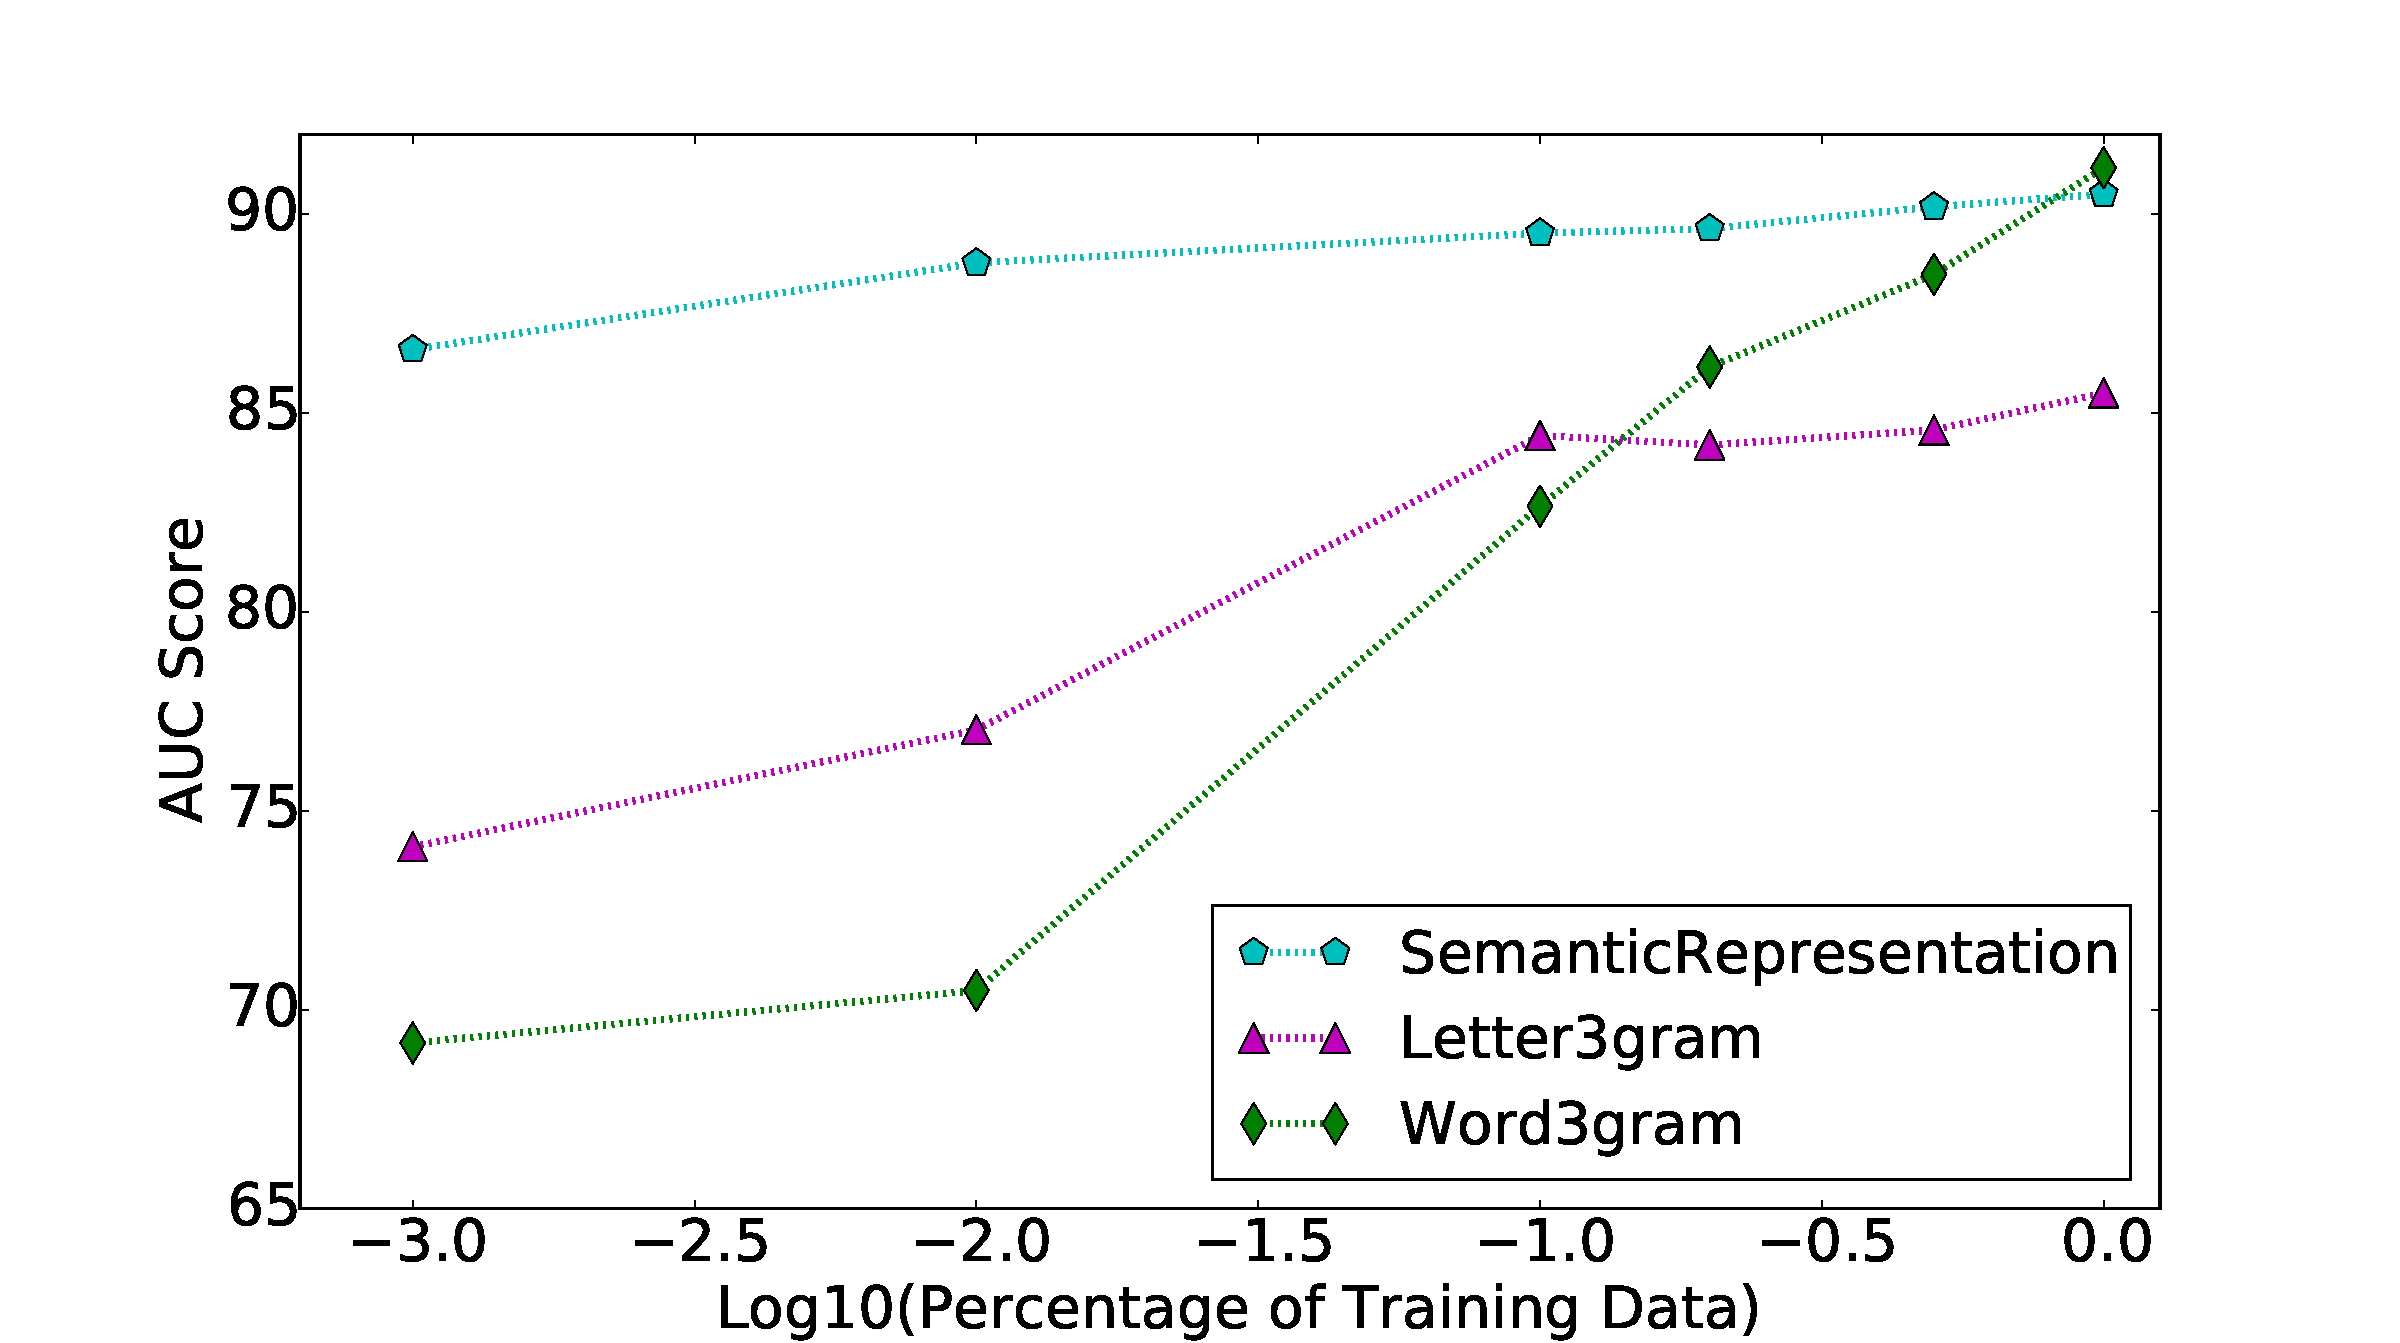
\includegraphics[scale=0.15]{figs/liu15multitask_hotel_svm}
%        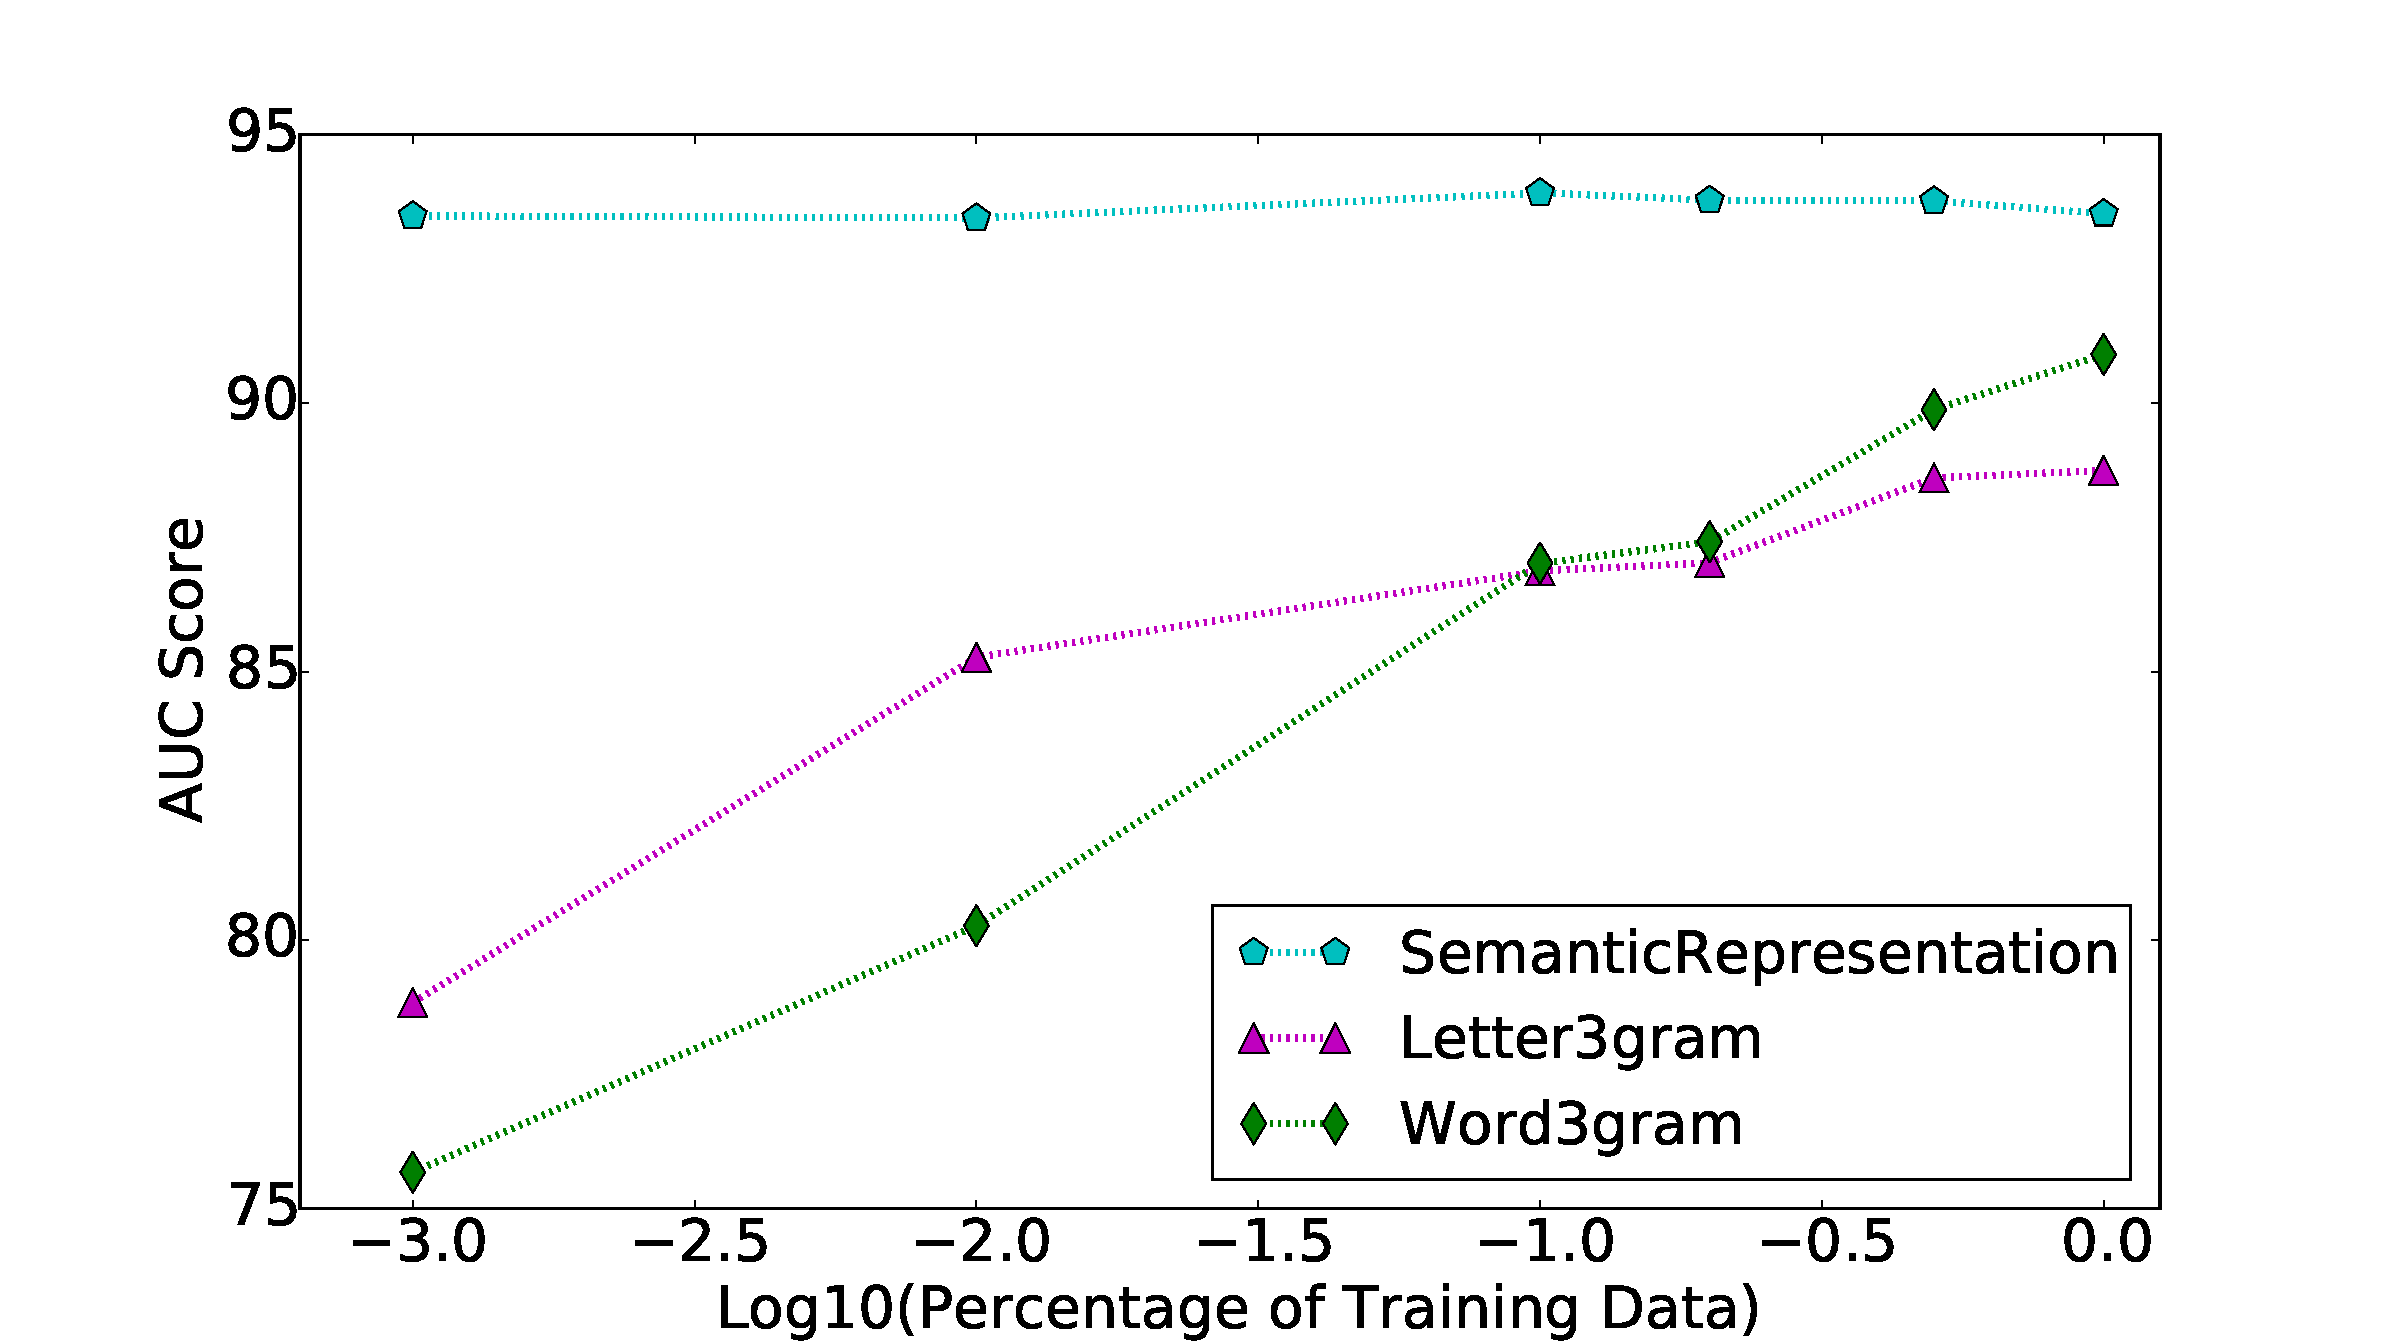
\includegraphics[scale=0.15]{figs/liu15multitask_flight_svm}\\
%        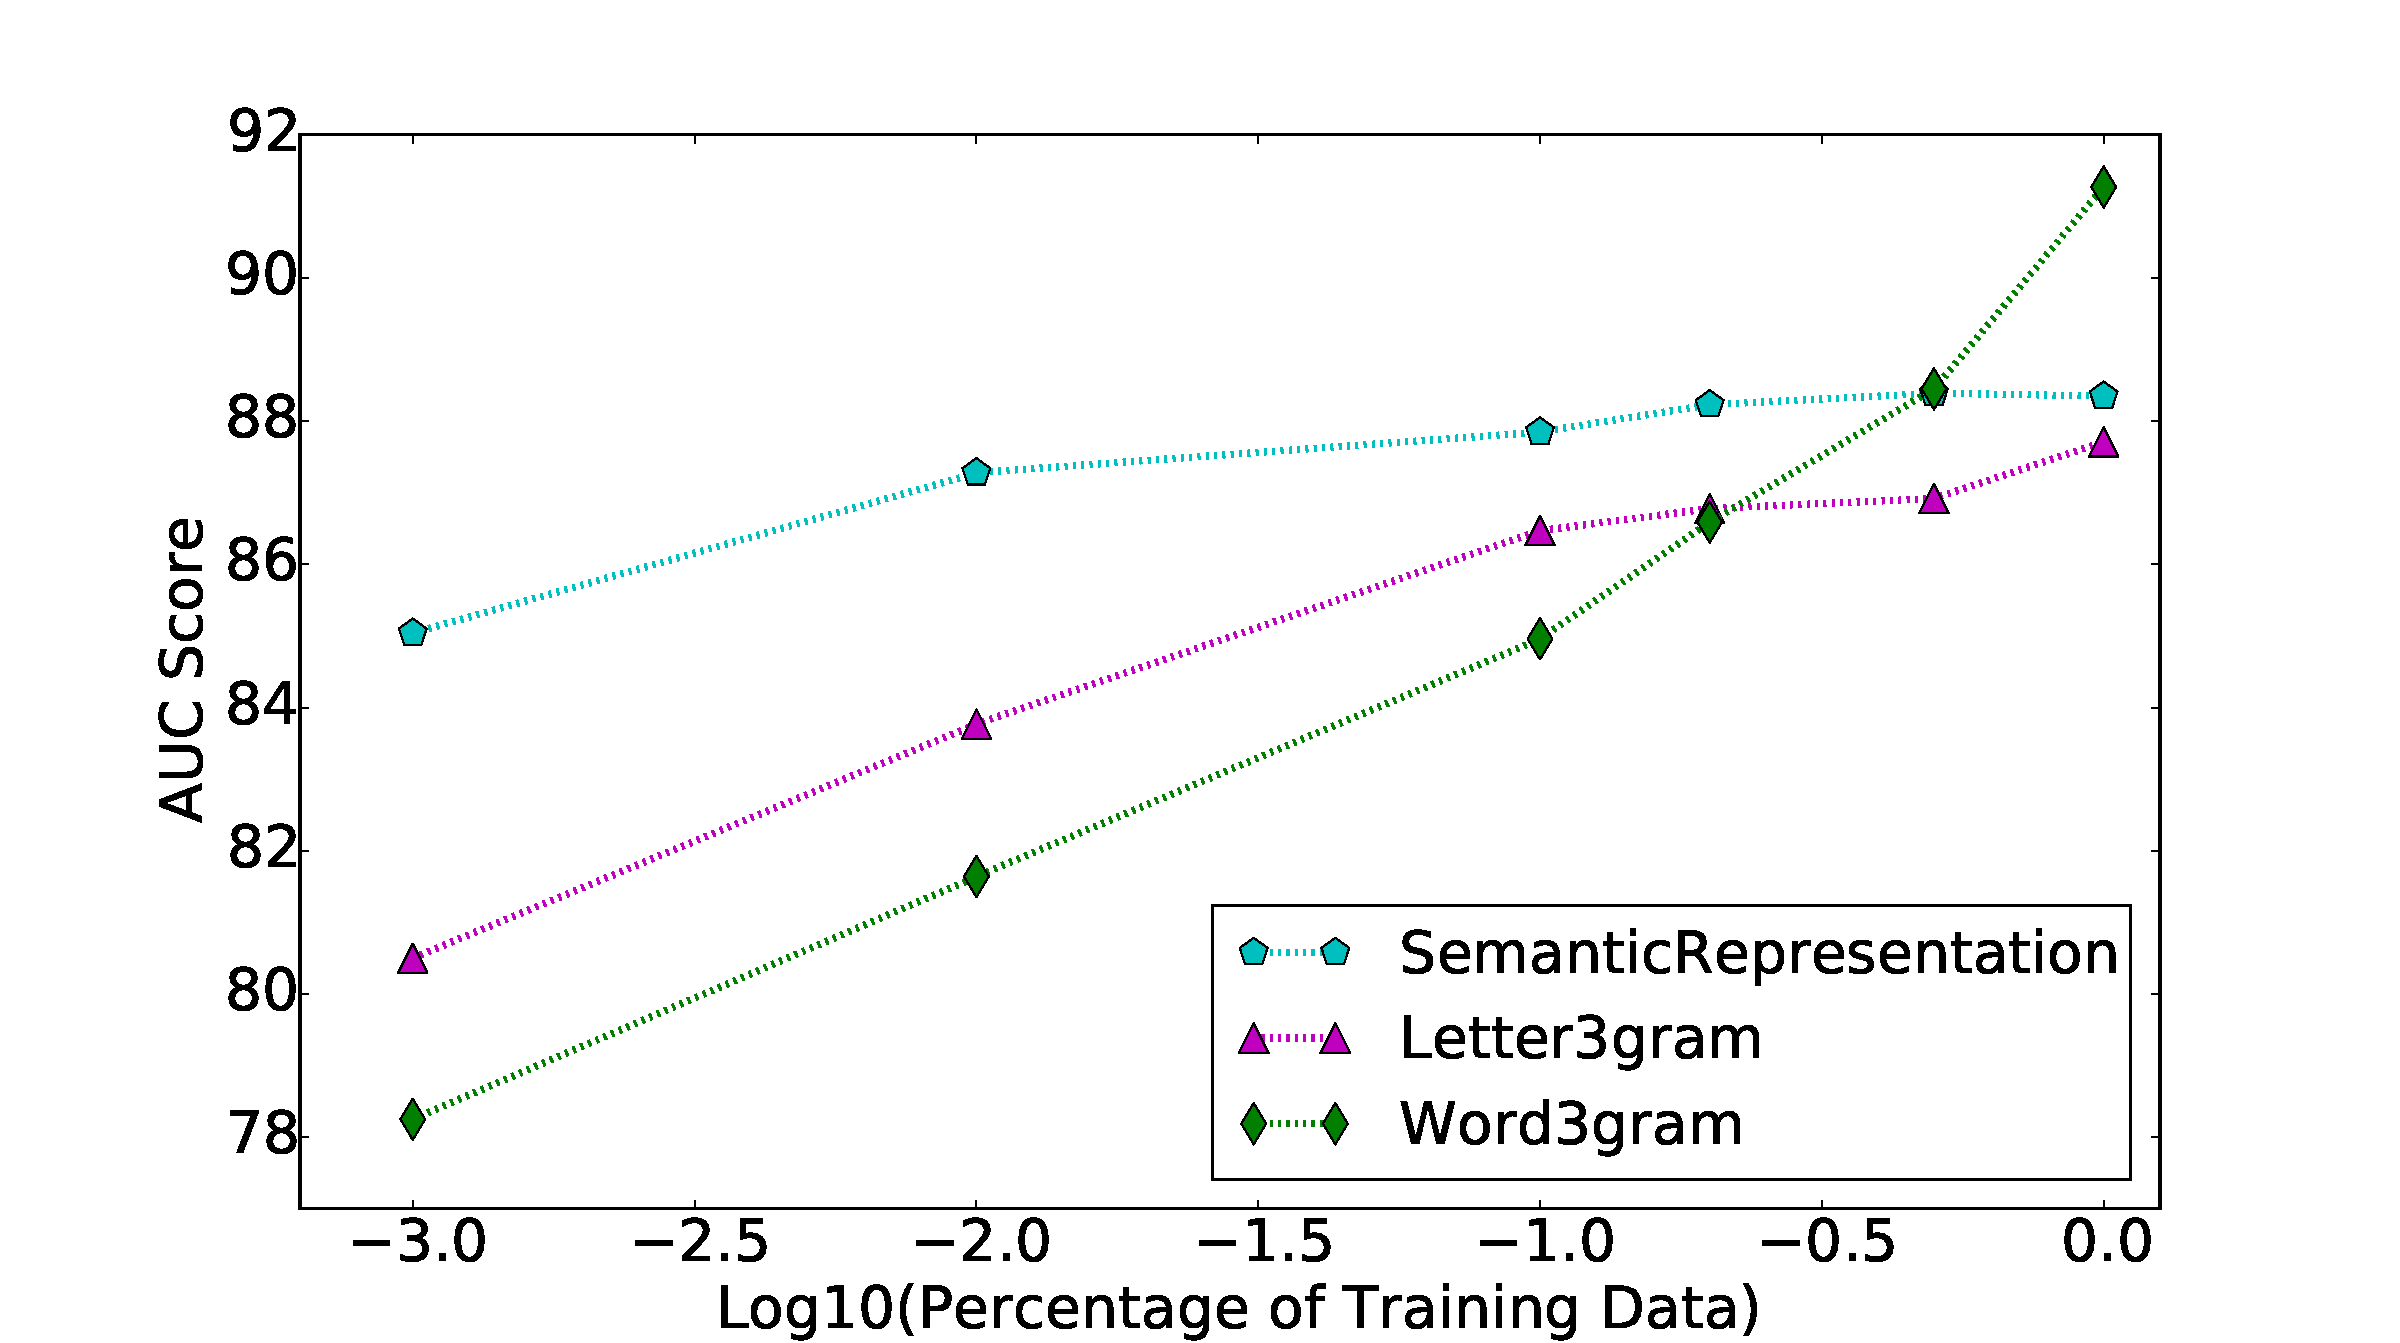
\includegraphics[scale=0.15]{figs/liu15multitask_restaurant_svm}
%        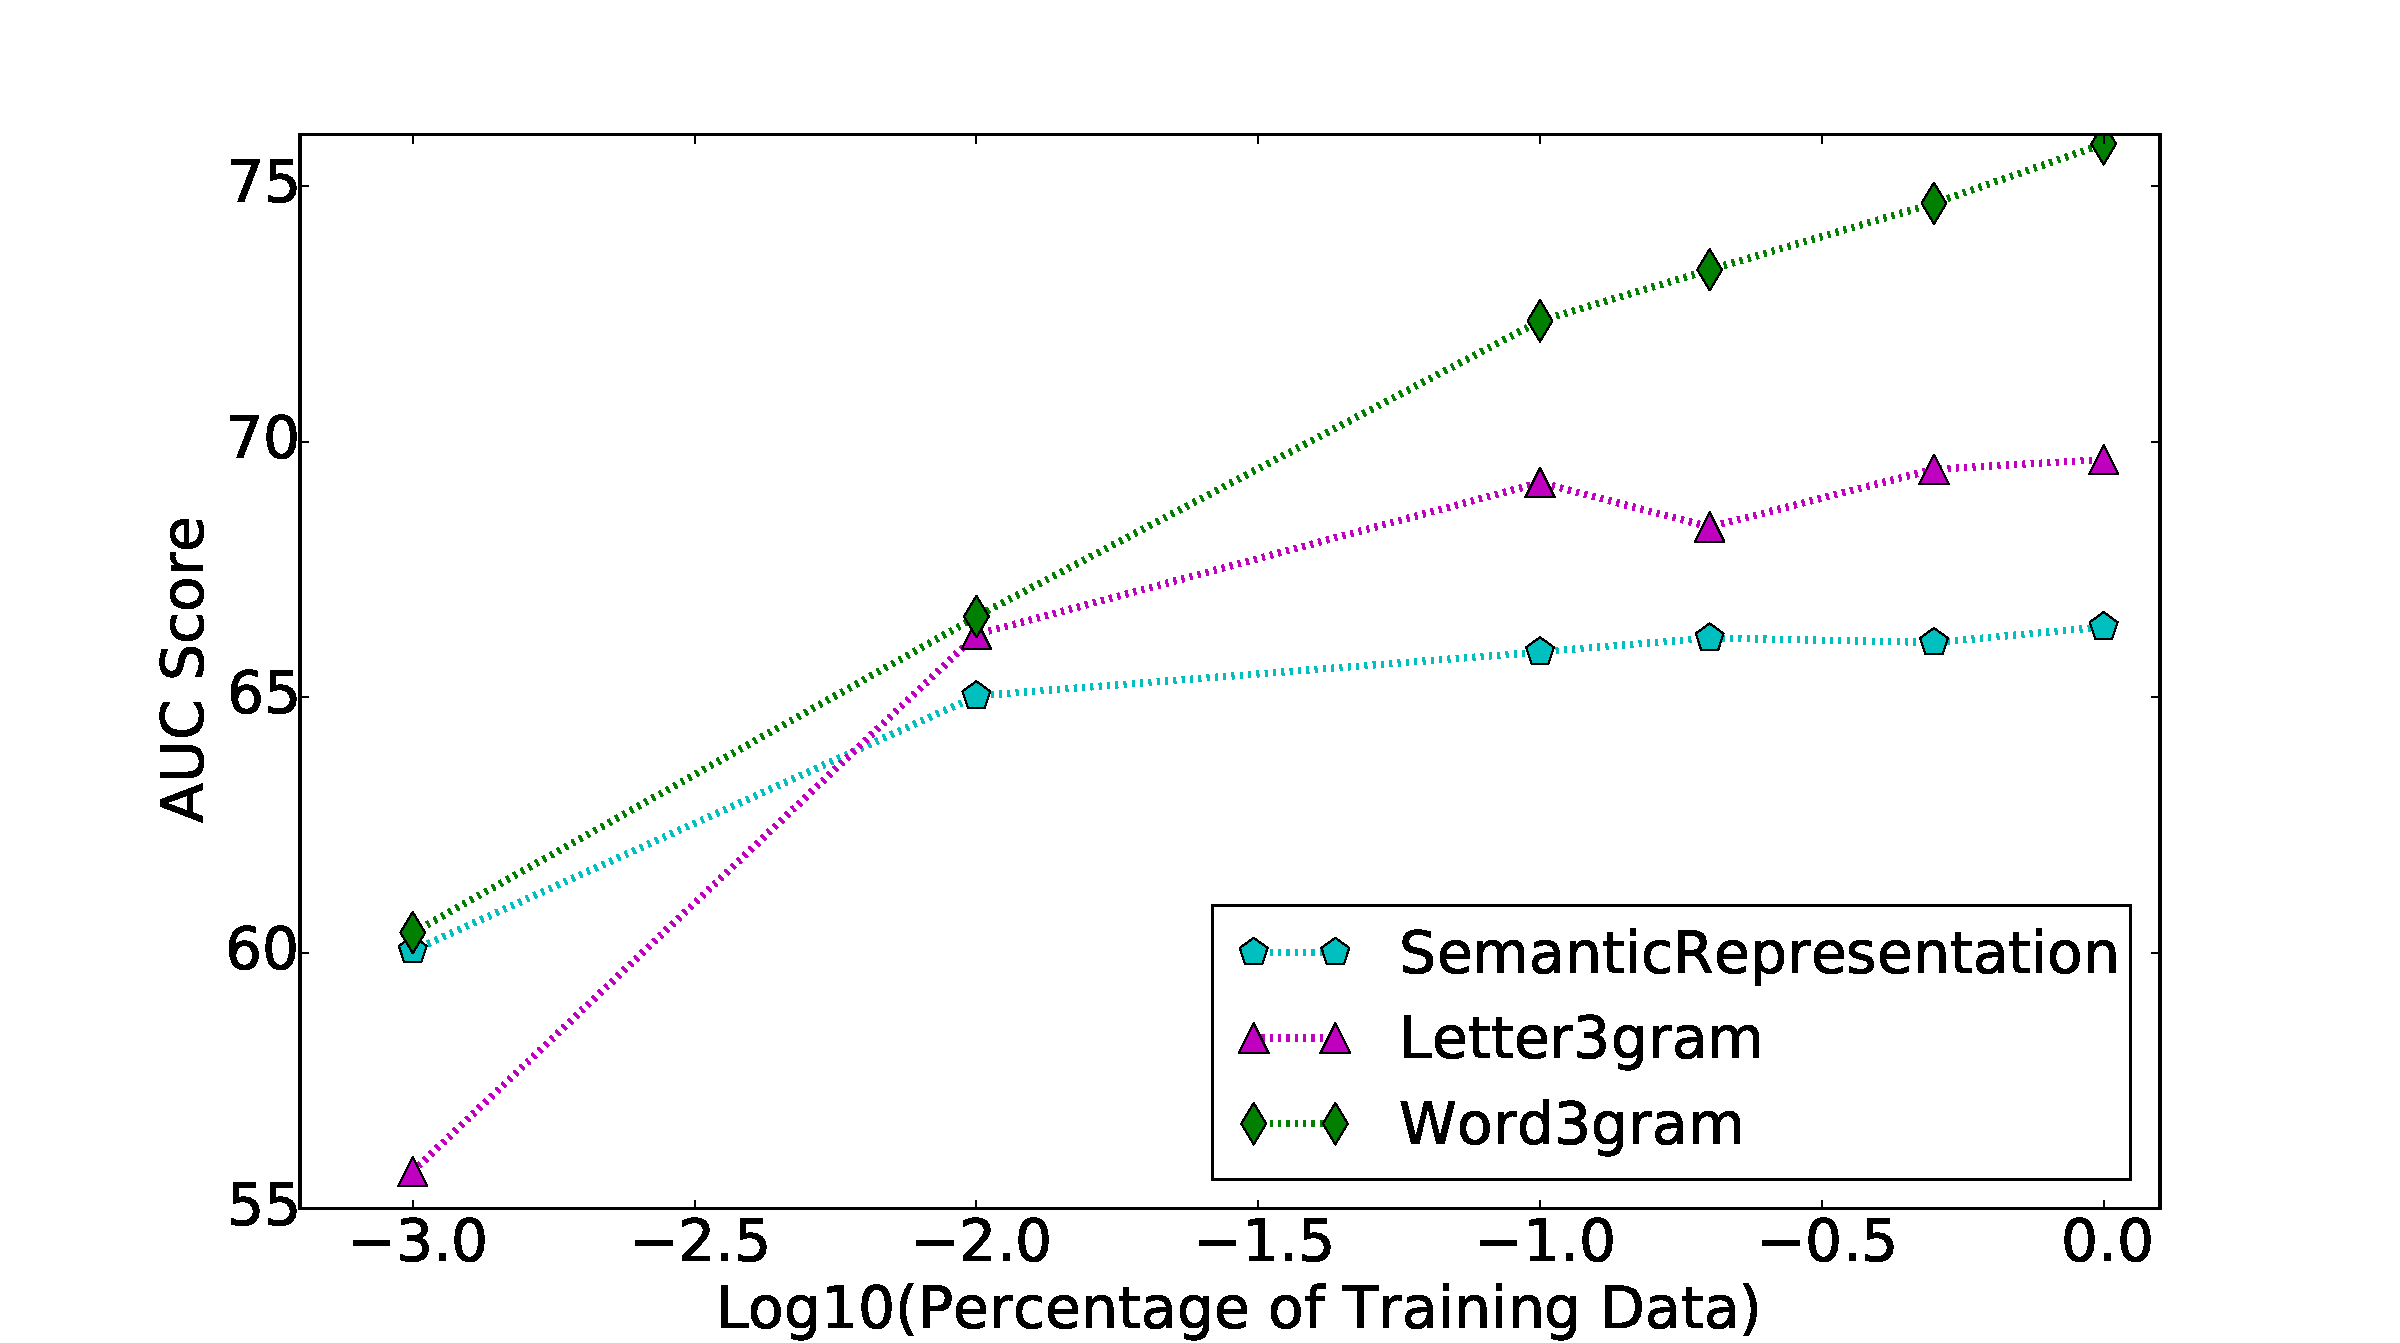
\includegraphics[scale=0.15]{figs/liu15multitask_nightlife_svm}
%
%\end{frame}


%% SUBSECTION%%%%%
\subsection[Infrastructure]{Computational Infrastructure}

%%%%%%
\begin{frame}
\frametitle{A note on Computational Infrastructure}
\bi
\pause
\item We always do our best: use biggest computer and largest dataset
\pause 
\item Don't pre-maturely performance-optimize your code/hardware
	\bi
	\item But be aware of ongoing efforts: \cite{coates13cots,dean12distributed} %TODO newer cites
	\ei
\pause
\item Invest in hyper-parameter tuning
	\bi
	\item Personal preference: I'd choose 10 low-end GeForce GPUs in favor of 1 high-end Tesla GPU to run more tuning experiments in parallel
	\ei
\ei
\end{frame}

\begin{frame}
\frametitle{Lots of hyper-parameters!}
\be
\item Number of layers
\item Number of nodes per layer
\item SGD learning rate
\item Detailed configurations of optimization method
\item Regularization constant
\item Mini-batch size
\item Type of non-linearity
\item Type of distribution for random initialization
\ee
\vspace{1cm}
Important to invest in finding good settings for {\color{red} your data}
\bi
        \item difference between a winning system vs. useless system
\ei
\end{frame}

\begin{frame}
\frametitle{Approaches to hyper-parameter tuning}
\be
\item Exhaustive grid search
\pause
\item Intelligent manual search, a.k.a Graduate Student Descent (GSD)
\pause
\item Treat as a meta machine learning problem \cite{bergstra11hyperparam}
	\bi
        \item Input $x$ = space of hyper-parameters
        \item Output $y$ = validation error after training with given hyper-parameters
        \pause
        \item Computing $y$ is expensive, so we learn a function f(x) that can predict it based on past $(x,y)$ pairs
        		\bi
	        \item e.g. Gaussian Process \cite{bergstra11hyperparam}, Evolutionary Algorithms \cite{moriya15automation}
	        \ei
	\ei
\ee
\pause

Future research: {\color{green} Green Learning}
\bi 
\item energy-efficient \& environmentally-friendly training procedures 
\item someone, please work on this!
\ei
\end{frame}

%%%%%%
\begin{frame}
\frametitle{Section Summary}
\centerline{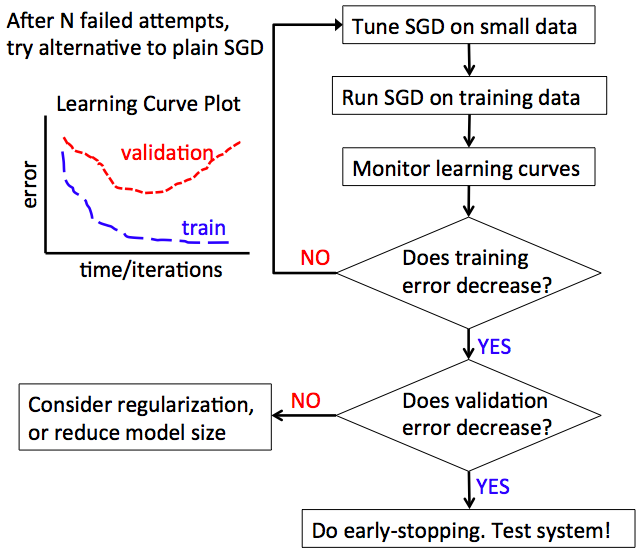
\includegraphics[scale=0.42]{figs/training_recipe}}
\end{frame}


